% Author: Xu Chen, University of Washington
% Lab 05 homework scene: robot R2 (taller, heavier, larger wheels) with Bluetooth telemetry; only what the
% homework gives (team gains, torque limit, delays); p and b0 are to be identified.
\documentclass[border=4pt]{standalone}
% Author: Xu Chen, University of Washington
% Shared TikZ style for the Control in Practice scene figures. % Author: Xu Chen, University of Washington
% Shared TikZ style for the Control in Practice scene figures. % Author: Xu Chen, University of Washington
% Shared TikZ style for the Control in Practice scene figures. \input{../../../docs/figures/cipstyle} from a lab.
\usepackage{amsmath,amssymb}
\usepackage[T1]{fontenc}
\usepackage{lmodern}
\usepackage{tikz}
\usepackage[siunitx]{circuitikz}
\usetikzlibrary{arrows.meta,calc,positioning,decorations.pathmorphing,decorations.markings,patterns,shapes.geometric,shadings,fit,backgrounds}
% restrained palette
\definecolor{ink}{HTML}{1A1A1A}
\definecolor{steel}{HTML}{8C96A0}
\definecolor{metal}{HTML}{D5DAE0}
\definecolor{accent}{HTML}{1F4E79}   % controller, signals we choose
\definecolor{plantc}{HTML}{FBE7D6}   % plant fill
\definecolor{sensorc}{HTML}{DCE8F3}  % sensor fill
\definecolor{dist}{HTML}{B03A2E}     % disturbances, forces from the environment
\definecolor{act}{HTML}{2E7D4F}      % actuation
\definecolor{note}{HTML}{555555}
\tikzset{
  every picture/.style={line width=0.8pt, >={Stealth[length=2.4mm]}, font=\small},
  thin line/.style={line width=0.5pt},
  thick line/.style={line width=1.2pt},
  dim/.style={thin line, note, {Stealth[length=1.6mm]}-{Stealth[length=1.6mm]}},
  ground/.style={pattern=north east lines, pattern color=steel, draw=none},
  block/.style={draw=ink, rounded corners=1.5pt, minimum height=9mm, minimum width=16mm, align=center, fill=white},
  plant/.style={block, fill=plantc},
  sensor/.style={block, fill=sensorc},
  ctrl/.style={block, draw=accent, text=accent, thick line},
  sum/.style={draw=ink, circle, minimum size=5mm, inner sep=0pt},
  sig/.style={->, ink},
  distsig/.style={->, dist, thick line},
  force/.style={-{Stealth[length=3mm]}, thick line},
  panel title/.style={font=\normalsize\bfseries, anchor=west, ink},
  caption/.style={font=\footnotesize, note, align=left},
}
 from a lab.
\usepackage{amsmath,amssymb}
\usepackage[T1]{fontenc}
\usepackage{lmodern}
\usepackage{tikz}
\usepackage[siunitx]{circuitikz}
\usetikzlibrary{arrows.meta,calc,positioning,decorations.pathmorphing,decorations.markings,patterns,shapes.geometric,shadings,fit,backgrounds}
% restrained palette
\definecolor{ink}{HTML}{1A1A1A}
\definecolor{steel}{HTML}{8C96A0}
\definecolor{metal}{HTML}{D5DAE0}
\definecolor{accent}{HTML}{1F4E79}   % controller, signals we choose
\definecolor{plantc}{HTML}{FBE7D6}   % plant fill
\definecolor{sensorc}{HTML}{DCE8F3}  % sensor fill
\definecolor{dist}{HTML}{B03A2E}     % disturbances, forces from the environment
\definecolor{act}{HTML}{2E7D4F}      % actuation
\definecolor{note}{HTML}{555555}
\tikzset{
  every picture/.style={line width=0.8pt, >={Stealth[length=2.4mm]}, font=\small},
  thin line/.style={line width=0.5pt},
  thick line/.style={line width=1.2pt},
  dim/.style={thin line, note, {Stealth[length=1.6mm]}-{Stealth[length=1.6mm]}},
  ground/.style={pattern=north east lines, pattern color=steel, draw=none},
  block/.style={draw=ink, rounded corners=1.5pt, minimum height=9mm, minimum width=16mm, align=center, fill=white},
  plant/.style={block, fill=plantc},
  sensor/.style={block, fill=sensorc},
  ctrl/.style={block, draw=accent, text=accent, thick line},
  sum/.style={draw=ink, circle, minimum size=5mm, inner sep=0pt},
  sig/.style={->, ink},
  distsig/.style={->, dist, thick line},
  force/.style={-{Stealth[length=3mm]}, thick line},
  panel title/.style={font=\normalsize\bfseries, anchor=west, ink},
  caption/.style={font=\footnotesize, note, align=left},
}
 from a lab.
\usepackage{amsmath,amssymb}
\usepackage[T1]{fontenc}
\usepackage{lmodern}
\usepackage{tikz}
\usepackage[siunitx]{circuitikz}
\usetikzlibrary{arrows.meta,calc,positioning,decorations.pathmorphing,decorations.markings,patterns,shapes.geometric,shadings,fit,backgrounds}
% restrained palette
\definecolor{ink}{HTML}{1A1A1A}
\definecolor{steel}{HTML}{8C96A0}
\definecolor{metal}{HTML}{D5DAE0}
\definecolor{accent}{HTML}{1F4E79}   % controller, signals we choose
\definecolor{plantc}{HTML}{FBE7D6}   % plant fill
\definecolor{sensorc}{HTML}{DCE8F3}  % sensor fill
\definecolor{dist}{HTML}{B03A2E}     % disturbances, forces from the environment
\definecolor{act}{HTML}{2E7D4F}      % actuation
\definecolor{note}{HTML}{555555}
\tikzset{
  every picture/.style={line width=0.8pt, >={Stealth[length=2.4mm]}, font=\small},
  thin line/.style={line width=0.5pt},
  thick line/.style={line width=1.2pt},
  dim/.style={thin line, note, {Stealth[length=1.6mm]}-{Stealth[length=1.6mm]}},
  ground/.style={pattern=north east lines, pattern color=steel, draw=none},
  block/.style={draw=ink, rounded corners=1.5pt, minimum height=9mm, minimum width=16mm, align=center, fill=white},
  plant/.style={block, fill=plantc},
  sensor/.style={block, fill=sensorc},
  ctrl/.style={block, draw=accent, text=accent, thick line},
  sum/.style={draw=ink, circle, minimum size=5mm, inner sep=0pt},
  sig/.style={->, ink},
  distsig/.style={->, dist, thick line},
  force/.style={-{Stealth[length=3mm]}, thick line},
  panel title/.style={font=\normalsize\bfseries, anchor=west, ink},
  caption/.style={font=\footnotesize, note, align=left},
}

\begin{document}
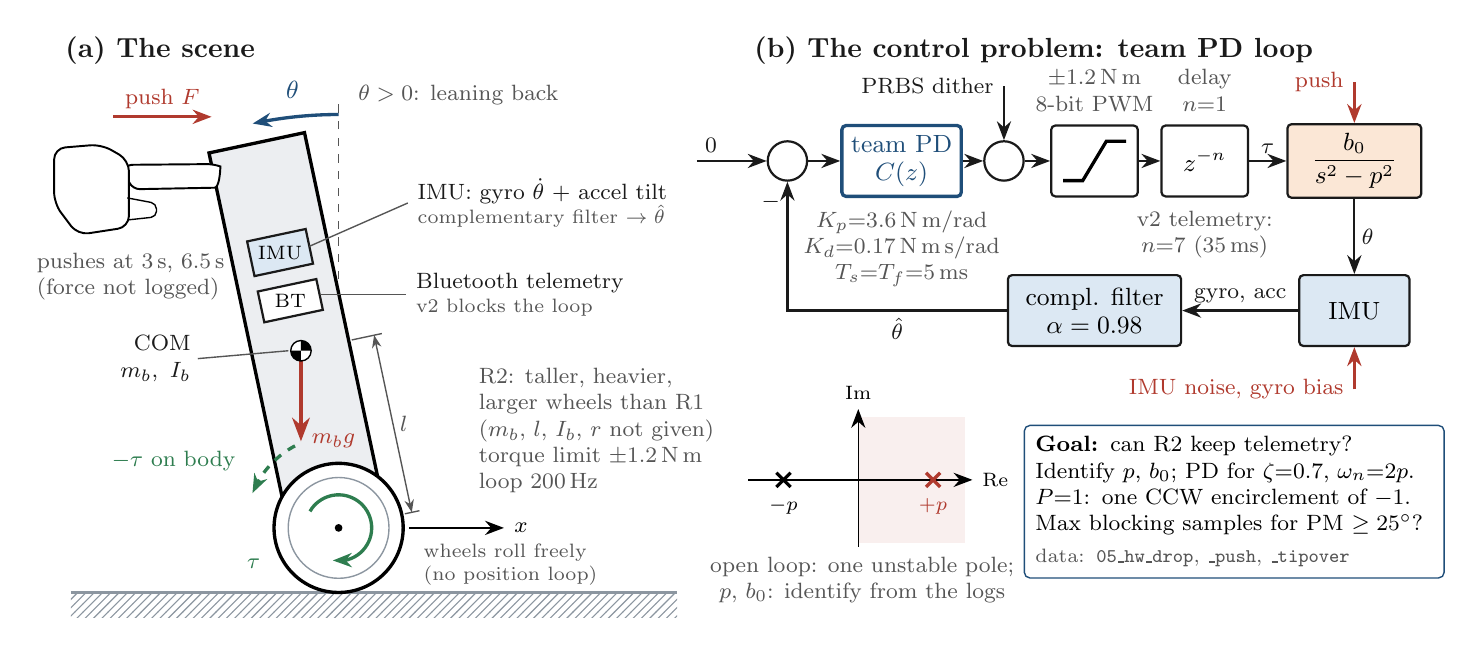
\begin{tikzpicture}
% ------------------------------------------------------------------ (a) the scene
\node[panel title] at (0,7.15) {(a) The scene};
\def\lean{12}
\coordinate (ax) at (3.6,1.09);
% floor
\fill[ground] (0.2,-0.05) rectangle (7.9,0.27);
\draw[thick line, steel] (0.2,0.27) -- (7.9,0.27);
% vertical reference through the axle
\draw[thin line, note, dashed] (ax) -- ++(0,5.4);
\begin{scope}[shift={(ax)}, rotate=\lean]
  % body (chassis box with battery, boards)
  \draw[fill=metal!45, thick line] (-0.62,-0.25) rectangle (0.62,5.0);
  % Bluetooth telemetry module
  \draw[fill=white, draw=ink] (-0.38,2.75) rectangle (0.38,3.15); \node[font=\scriptsize] at (0,2.95) {BT};
  \coordinate (bt) at (0.38,2.95);
  % IMU board
  \draw[fill=sensorc, draw=ink] (-0.38,3.35) rectangle (0.38,3.8);
  \node[font=\scriptsize] at (0,3.575) {IMU};
  \coordinate (imu) at (0.38,3.575);
  % COM
  \coordinate (com) at (0,2.3);
  \coordinate (push) at (-0.62,4.6);
  % l dimension along the right face
  \draw[dim] (0.95,0) -- node[right=-1pt, font=\footnotesize] {$l$} (0.95,2.3);
  \draw[thin line, note] (0.86,0) -- (1.05,0) (0.66,2.3) -- (1.05,2.3);
\end{scope}
% wheel (in front of the body)
\draw[thick line, fill=white] (ax) circle (0.82);
\draw[thin line, steel] (ax) circle (0.64);
\fill (ax) circle (1.4pt);
% COM symbol and gravity
\draw[dist, force] (com) -- ++(0,-1.15) node[right=0pt, font=\footnotesize] {$m_b g$};
\fill[white] (com) circle (0.13); \draw[thin line] (com) circle (0.13);
\fill (com) -- ++(0.13,0) arc (0:90:0.13) -- cycle;
\fill (com) -- ++(-0.13,0) arc (180:270:0.13) -- cycle;
\draw[thin line, note] (com) ++(-0.16,0) -- ++(-1.15,-0.1) node[left=-1pt, font=\footnotesize, ink, align=right] {COM\\$m_b,\ I_b$};
% pitch angle
\draw[->, accent, thick line] ($(ax)+(90:5.25)$) arc (90:90+\lean:5.25);
\node[accent] at ($(ax)+(90+\lean/2:5.6)$) {$\theta$};
\node[caption, anchor=west] at ($(ax)+(0.12,5.5)$) {$\theta>0$: leaning back};
% wheel torque on the wheel (drives it forward, +x) and reaction on the body
\draw[act, thick line, ->] ($(ax)+(150:0.42)$) arc (150:-100:0.42);
\node[act, font=\footnotesize] at ($(ax)+(-1.08,-0.45)$) {$\tau$};
\draw[act, thick line, ->, dashed] ($(ax)+(118:1.18)$) arc (118:158:1.18);
\node[act, font=\footnotesize, anchor=east] at ($(ax)+(-1.18,0.85)$) {$-\tau$ on body};
% wheel coordinate
\draw[->] ($(ax)+(0.9,0)$) -- ++(1.2,0) node[right, font=\footnotesize] {$x$};
\node[caption, anchor=north west, font=\scriptsize] at ($(ax)+(0.95,-0.08)$) {wheels roll freely\\(no position loop)};
% IMU callout
\draw[thin line, note] (imu) -- ++(1.25,0.55) node[right, font=\footnotesize, ink, align=left]
  {IMU: gyro $\dot\theta$ + accel tilt\\[-1pt]\scriptsize\color{note}complementary filter $\to\hat\theta$};
\draw[thin line, note] (bt) -- ++(1.1,0.0) node[right, font=\footnotesize, ink, align=left]
  {Bluetooth telemetry\\[-1pt]\scriptsize\color{note}v2 blocks the loop};
% finger / hand pushing at the top (forward push, +x)
\begin{scope}[shift={(push)}]
  \draw[fill=white, line width=0.7pt, rounded corners=2.5pt]
    (0,-0.05) -- (-1.05,-0.07) -- (-1.15,0.12) -- (-1.15,0.24) -- (-0.02,0.25) .. controls (0.06,0.22) and (0.06,0.0) .. (0,-0.05);
  \draw[fill=white, line width=0.7pt, rounded corners=4pt]
    (-1.1,0.3) -- (-1.1,-0.55) -- (-1.75,-0.65) -- (-2.05,-0.25) -- (-2.05,0.45) -- (-1.45,0.5) -- cycle;
  \draw[thin line, rounded corners=2pt] (-1.12,-0.18) -- (-0.75,-0.25) -- (-0.75,-0.42) -- (-1.12,-0.46);
  \draw[distsig] (-1.3,0.85) -- (-0.05,0.85) node[midway, above=-1pt, font=\footnotesize] {push $F$};
\end{scope}
\node[caption, anchor=north west] at ($(push)+(-2.4,-0.75)$) {pushes at 3\,s, 6.5\,s\\(force not logged)};
% parameters and log
\node[caption, anchor=north west] at (5.25,3.25) {R2: taller, heavier,\\larger wheels than R1\\($m_b$, $l$, $I_b$, $r$ not given)\\torque limit $\pm1.2$\,N\,m\\loop 200\,Hz};

% ------------------------------------------------------------------ (b) the control problem
\begin{scope}[shift={(8.75,0)}]
\node[panel title] at (0,7.15) {(b) The control problem: team PD loop};
\def\ya{5.75} \def\yb{3.85}
\node[sum] (s1) at (0.55,\ya) {};
\node[ctrl, minimum width=14mm] (pd) at (2.0,\ya) {team PD\\[-1pt]$C(z)$};
\node[sum] (s2) at (3.3,\ya) {};
\node[block, minimum width=11mm] (sat) at (4.45,\ya) {};
\draw[thick line] ($(sat)+(-0.4,-0.25)$) -- ($(sat)+(-0.15,-0.25)$) -- ($(sat)+(0.15,0.25)$) -- ($(sat)+(0.4,0.25)$);
\node[block, minimum width=11mm] (del) at (5.85,\ya) {$z^{-n}$};
\node[plant, minimum width=17mm] (G) at (7.75,\ya) {$\dfrac{b_0}{s^2-p^2}$};
\node[sensor, minimum width=14mm] (imu) at (7.75,\yb) {IMU};
\node[sensor, minimum width=22mm] (cf) at (4.45,\yb) {compl. filter\\[-1pt]$\alpha=0.98$};
\draw[sig] (-0.6,\ya) node[above right=-1pt, font=\footnotesize] {$0$} -- (s1);
\draw[sig] (s1) -- (pd);
\draw[sig] (pd) -- (s2);
\draw[sig] (s2) -- (sat);
\draw[sig] (sat) -- (del);
\draw[sig] (del) -- node[above=-1pt, font=\footnotesize] {$\tau$} (G);
\draw[sig] (G) -- node[right=-1pt, font=\footnotesize] {$\theta$} (imu);
\draw[sig] (imu) -- node[above=-1pt, font=\footnotesize] {gyro, acc} (cf);
\draw[sig] (cf) -| node[pos=0.25, below=-1pt, font=\footnotesize] {$\hat\theta$} node[pos=0.92, left=-1pt, font=\footnotesize] {$-$} (s1);
% inputs: dither, push, IMU noise
\draw[sig] (3.3,\ya+0.95) node[left, font=\footnotesize] {PRBS dither} -- (s2);
\draw[distsig] (7.75,\ya+1.0) node[left, font=\footnotesize, dist] {push} -- (G);
\draw[distsig] (7.75,\yb-1.0) node[left, font=\footnotesize, dist] {IMU noise, gyro bias} -- (imu);
% annotations
\node[caption, anchor=north, align=center] at (2.0,\ya-0.5) {$K_p{=}3.6$\,N\,m/rad\\$K_d{=}0.17$\,N\,m\,s/rad\\$T_s{=}T_f{=}5$\,ms};
\node[caption, anchor=south, align=center] at (4.45,\ya+0.5) {$\pm1.2$\,N\,m\\8-bit PWM};
\node[caption, anchor=south, align=center] at (5.85,\ya+0.5) {delay\\$n{=}1$};
\node[caption, anchor=north, align=center] at (5.85,\ya-0.5) {v2 telemetry:\\$n{=}7$ (35\,ms)};
% s-plane inset: one unstable pole
\begin{scope}[shift={(1.45,1.7)}]
  \fill[dist!8] (0,-0.8) rectangle (1.35,0.8);
  \draw[->, thin line] (-1.4,0) -- (1.45,0) node[right, font=\scriptsize] {Re};
  \draw[->, thin line] (0,-0.85) -- (0,0.9) node[above, font=\scriptsize] {Im};
  \draw[thick line] (-0.95,0) ++(-0.09,-0.09) -- ++(0.18,0.18) ++(0,-0.18) -- ++(-0.18,0.18);
  \draw[thick line, dist] (0.95,0) ++(-0.09,-0.09) -- ++(0.18,0.18) ++(0,-0.18) -- ++(-0.18,0.18);
  \node[font=\scriptsize, below] at (-0.95,-0.1) {$-p$};
  \node[font=\scriptsize, below, dist] at (0.95,-0.1) {$+p$};
  \node[caption, anchor=north, align=center] at (0.05,-0.85) {open loop: one unstable pole;\\$p$, $b_0$: identify from the logs};
\end{scope}
% goal / data box
\node[draw=accent, thin line, rounded corners=2pt, fill=white, align=left, anchor=north west, font=\footnotesize,
      text width=5.05cm, inner sep=4pt] at (3.55,2.4)
  {\textbf{Goal:} can R2 keep telemetry?\\
   Identify $p$, $b_0$; PD for $\zeta{=}0.7$, $\omega_n{=}2p$.\\
   $P{=}1$: one CCW encirclement of $-1$.\\
   Max blocking samples for PM $\ge25^\circ$?\\[2pt]
   {\scriptsize\color{note}data: \texttt{05\_hw\_drop}, \texttt{\_push}, \texttt{\_tipover}}};
\end{scope}
\end{tikzpicture}
\end{document}
